\section{Fading}\label{sc:fading}
The above plots all give a good estimate of the RSSI in a stationary clean environment with stationary nodes, but in case of a dynamic environment with obstacles, concepts like fading must be considered. Intrinsic and extrinsic electronic noise set the signal to noise ratio floor of the received signal, but more expensive electronics can compensate for the former noise source, and say no mobile phones at the racetrack can lead to less of the latter noise source, however the RSSI still will experience signal strength drops at times in a dynamic environment. The broadcasting behaviour of the wireless sensor network causes constructive and destructive interference at the receiver, which can lead to deep fading. Deep fading is the scenario in which two or more, out of phase, adequate signals arrive at the receiver simultaneously, leading to a critical destructive interference. The deep fading interferences causes the signal strength to fall below the established noise floor, deeming the signal unreliable or unmeasurable. In the scenario a receiver has experienced a deep fade, depending on the time length, or number of lost packages, the scenario is characterised as a fast fade or a slow fade. This is typically cause by reflection, diffraction or scattering of the signal, causing in line of sight (LOS) signal interfering with a none line of sight (NLOS) signals. The moving of the nodes relative to each other not only has interference, but they have a change in behaviour also. An example of behaviour changing fading is the doppler fading, in which the signal tends to shift in frequency relative to the movement of the sink and the source node. 

\subsection{Doppler Fading}
Following the standard IEEE\_802.15.4, it permits the Telosb to transmit in the ISM  band at frequencies between $2.4$ and $2.4835 GHz$. Having 12 channels, $2 MHz$ wide and separated by $5 MHz$, the TelosB allows a centre frequency signal to shift $\pm 1 MHz$ while still being acknowledged by the receiving channel. Does the signal shift the frequency more than $1 MHz$, the receiving node will simply filter out the signal and the package will be lost. The sign of the shift in frequency depends on the distance between the source and the sink increasing or decreasing. The running node will be changing position relative to the base station at different speeds due to the shape of the track, so an investigation of the effect to the case was made. Firstly, the distance between a package, every quarter of a second, covered by a runner, running at $12kph$, was calculated closest and furthest on the track relative to the base station. The runner is running circular, but the change in distance experienced by the base station will by a straight line leading to doppler frequency found at different speeds relative to track position. The results showed a $29.698Hz$ frequency shift at the end of the track, while the at the top of the track a $26.773Hz$ shift happened. The buffer of $1MHz$ was far beyond the results needed for danger of lost packages due to doppler fading. Just for scalability and flexibility the extreme case was also calculated for the system. Had the runner been running the package distance at approximately $50000kph$ doppler fading would have been an issue. Given the calculated results the project is focusing on fast and slow fading as a simulated instead. See appendix 2 for doppler calculations.

\subsection{Fast Fading and Slow Fading}%TODO reference to appendix
Busty bit errors at the receiver is often measured in clusters with different duration or length. Fast fading clusters are typically in the range of tens to hundreds of milliseconds, before the received signal again is adequate, while slow fading clusters are in the range of tens of seconds to minutes. Fast fading and slow fading are both biproducts of the broadcasting behaviour of the nodes, while no clean separation can be made between the two, slow fading is referred to as a shadowing effect and fast fading can be simplified to reflection. E.g. a signal at $2.4GHz$ will have a wavelength of $12.5cm$, given an opposite phased signal every $12.5cm$. If the $2.4GHz$ LOS signal travels $1m$ to the sink and the NLOS signal travels $1.125m$ to the sink, they would cancel each other out. Unfortunately, the calculations of the reflected fading also must consider the directivity of the antenna, since the signal strength also varies at different angles from the source. An antenna with high directivity will since not have a full cancelation at the sink, since the LOS signal will have a higher amplitude than the NLOS signal. From [1, page 92] the drop-in signal strength can be estimated to be around $30-40dB$ ($60-70dBm$), and this is the values for both slow and fast fading chosen for the simulations in this project. Slow fading can represent diffraction and scattering of the signal from objects in between source and sink, e.g. more runners on the track or the photographer taking images along the route. The slow fading since is modelled as a random stochastic variable with a showing variance visualized through a lognormal fading plot. Given a shadowing variance of $2.22dBm$ and probability of occurrence at $10\%$ for both fast and slow fading, fast fading effect is simulated to last 333 milliseconds while slow fading is simulated to last 14seconds. Figure \ref{fig:logpathReceivedSignal_baseStation_baseOnly} plots the base station RSSI including fading, while Figure \ref{fig:binaryDeepFading_baseStation_baseOnly} plot the binary, received or lost package, output of the base station. Figure \ref{fig:logpathReceivedSignal_combinedStations_baseOnly} plots the combined stations RSSI including fading, while Figure \ref{fig:binaryDeepFading_combinedStations_baseOnly} plot the binary output of the combined stations and Figure \ref{fig:logpathReceivedSignal_combinedStations_allStations} and \ref{fig:binaryDeepFading_combinedStations_allStations} shows a combined stations plot, but with all three station signals being victims of individual fading patterns. 
\clearpage

%Figure 7, 8 and 9
\begin{figure}[H]
	\centering
	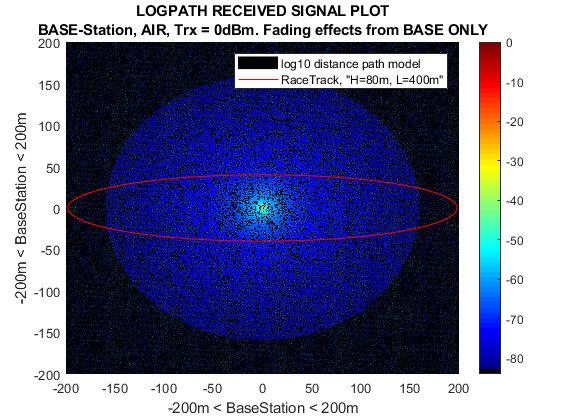
\includegraphics[width=\linewidth]{theory/fading/fig/logpathReceivedSignal_baseStation_baseOnly.png}
	\caption{Base Station RSSI plot after base station experiencing fading}
	\label{fig:logpathReceivedSignal_baseStation_baseOnly}
\end{figure}

\begin{figure}[H]
	\centering
	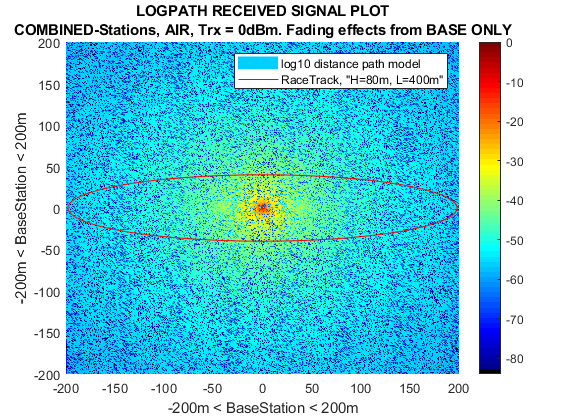
\includegraphics[width=\linewidth]{theory/fading/fig/logpathReceivedSignal_combinedStations_baseOnly.png}
	\caption{Combined Stations RSSI plot after base station experiencing fading}
	\label{fig:logpathReceivedSignal_combinedStations_baseOnly}
\end{figure}

\begin{figure}[H]
\centering
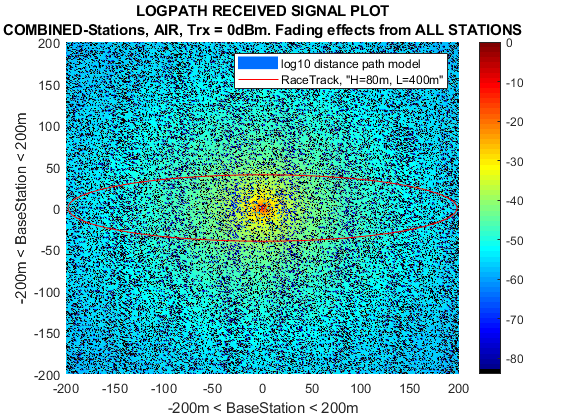
\includegraphics[width=\linewidth]{theory/fading/fig/logpathReceivedSignal_combinedStations_allStations.png}
\caption{Combined Stations RSSI plot after all stations experiencing fading}
\label{fig:logpathReceivedSignal_combinedStations_allStations}
\end{figure}

\begin{figure}[H]
	\centering
	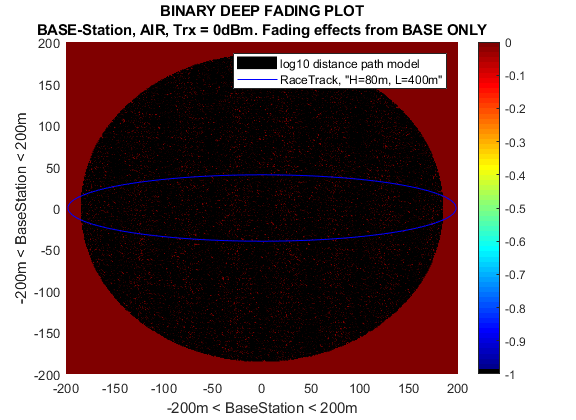
\includegraphics[width=\linewidth]{theory/fading/fig/binaryDeepFading_baseStation_baseOnly.png}
	\caption{Base Station Deep fading plot after base station experiencing fading}
	\label{fig:binaryDeepFading_baseStation_baseOnly}
\end{figure}

\begin{figure}[H]
	\centering
	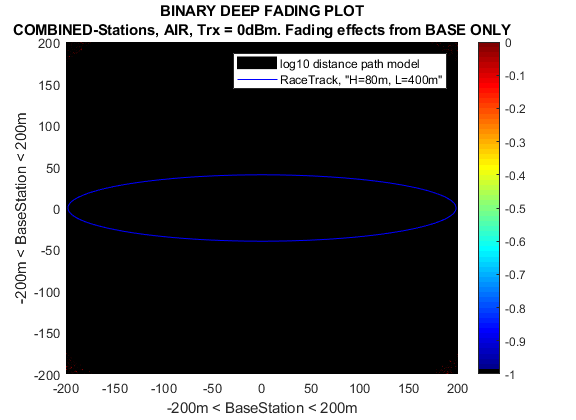
\includegraphics[width=\linewidth]{theory/fading/fig/binaryDeepFading_combinedStations_baseOnly.png}
	\caption{Combined Stations Deep fading plot after base station experiencing fading}
	\label{fig:binaryDeepFading_combinedStations_baseOnly}
\end{figure}

\begin{figure}[H]
	\centering
	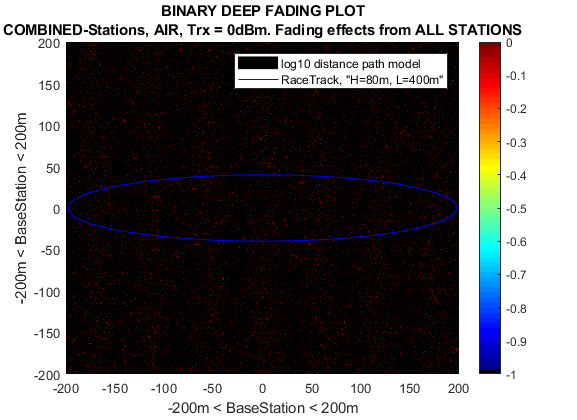
\includegraphics[width=\linewidth]{theory/fading/fig/binaryDeepFading_combinedStations_allStations.png}
	\caption{Combined Stations Deep fading plot after all stations experiencing fading}
	\label{fig:binaryDeepFading_combinedStations_allStations}
\end{figure}

